% Onpersoonlijk:
\section{Planning} \label{planning}
De planning wordt beheerd via GitHub en omvat drie verschillende weergaven: Overview, ToDoList en roadmap.

In de \textbf{Overview}\textit{(zie figuur \ref{fig:overview})} wordt een samenvatting van alle taken getoond, inclusief de voltooide en de nog uit te voeren taken. Deze samenvatting omvat de volgende informatie:

    \textit{Repository}: Het project waaraan de taak is gekoppeld.\\
    \textit{Titel}: De naam van de opdracht.\\
    \textit{Assignees}: Verantwoordelijke personen voor de uitvoering van de opdracht.\\
    \textit{Status}: De voortgang van de opdracht.\\
    \textit{Startdatum en Deadline}: De begin- en einddatum van de opdracht.\\
    \textit{Prioriteit}: De urgentie van de opdracht.\\

\begin{figure}[h]
\centering
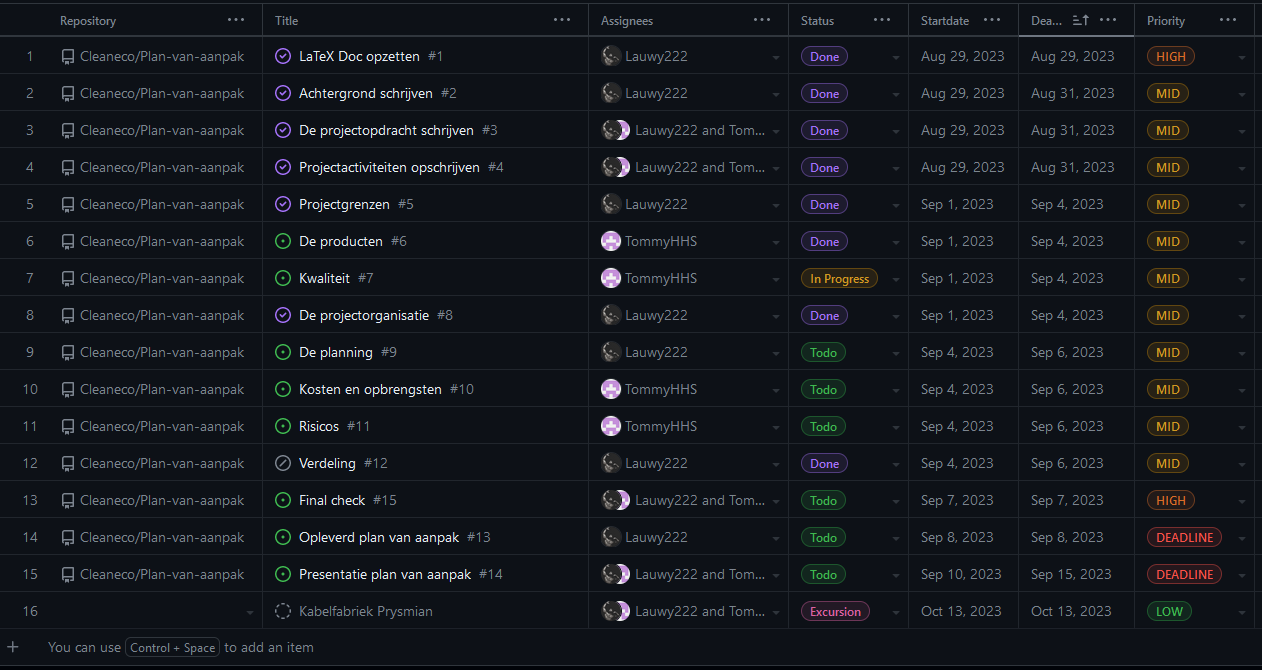
\includegraphics[width=0.9\textwidth]{IMG/overview.PNG}
\caption{Screenshot van de Overview in GitHub.}
\label{fig:overview}
\end{figure}

\newpage

In de \textbf{ToDoList}\textit{(zie figuur \ref{fig:todolist})} worden vier lijsten weergegeven en onderverdeeld onder vier categorieën: Te doen, In uitvoering, Voltooid en Excursie. Hier wordt aangegeven in welke fase van voltooiing elke opdracht zich bevindt, of deze nog moet worden uitgevoerd, in uitvoering is, is voltooid of betrekking heeft op een excursie die moet worden voorbereid.

\begin{figure}[h]
\centering
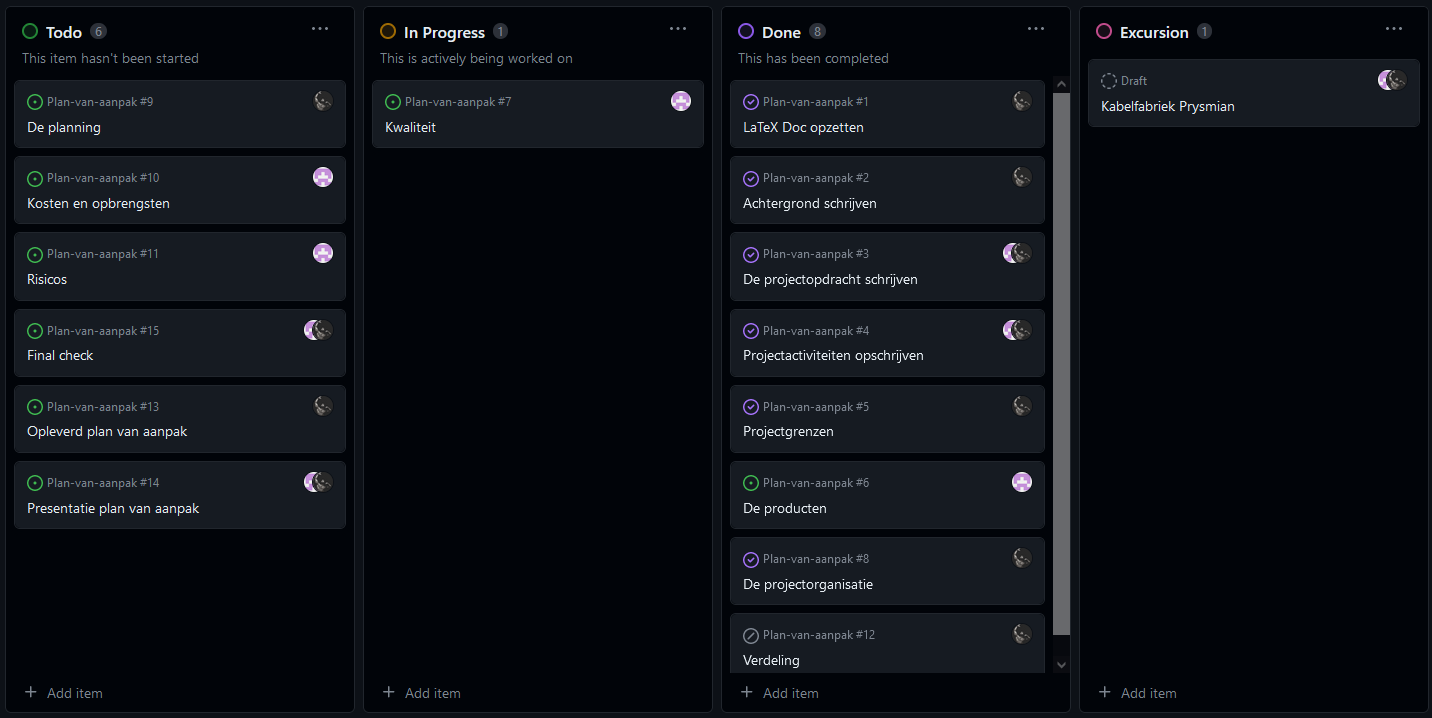
\includegraphics[width=0.9\textwidth]{IMG/todolist.PNG}
\caption{Screenshot van de ToDoList in GitHub.}
\label{fig:todolist}
\end{figure}

De \textbf{Roadmap}\textit{(zie figuur \ref{fig:roadmap})} biedt een visuele weergave van wanneer elke opdracht gepland was om te beginnen en wanneer de deadline is.

\begin{figure}[h]
\centering
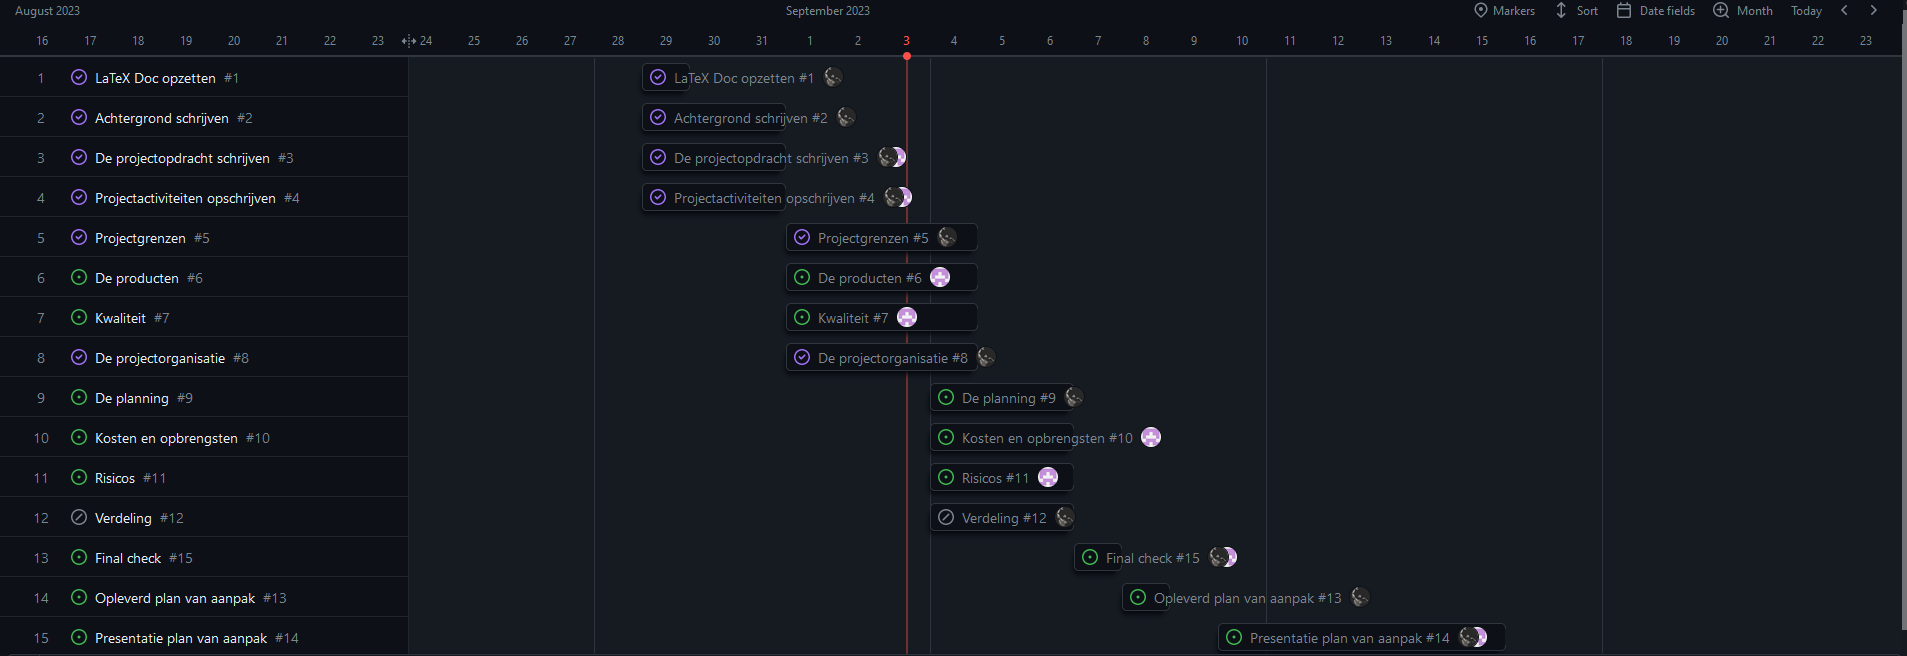
\includegraphics[width=0.9\textwidth]{IMG/roadmap.PNG}
\caption{Screenshot van de Roadmap in GitHub.}
\label{fig:roadmap}
\end{figure}

Indien er complicaties optreden tijdens het verloop van dit project, kunnen er tijdig opmerkingen worden geplaatst en om assistentie worden gevraagd. Hierdoor is er geen noodzaak voor fysieke vergaderingen en kan per opdracht aangegeven worden welke problemen zich voordoen en wat de projectstructuur nog verder verbetert.

% % SEMINEW
% \section{Planning} \label{planning}
% We gebruiken de Github planning met drie verschillende weergaven: Overview, ToDoList en roadmap.

% In het \textbf{Overview}\textit{(figuur:\ref{fig:overview})} tonen we een samenvatting van alle taken, inclusief degenen die zijn voltooid of nog moeten worden uitgevoerd, met devolgende informatie:

% - \textit{Repository}: Aan welk project het onderwerp is gekoppeld\\
% - \textit{Titel}: De naam van de opdracht\\
% - \textit{Assignees}: Wie verantwoordelijk is voor het uitvoeren van de opdracht\\
% - \textit{Status}: De voortgang van de opdracht\\
% - \textit{Startdatum} en Deadline: De begin- en einddatum van de opdracht\\
% - \textit{Prioriteit}: De urgentie van de opdracht\\

% \begin{figure}[h]
%     \centering
%     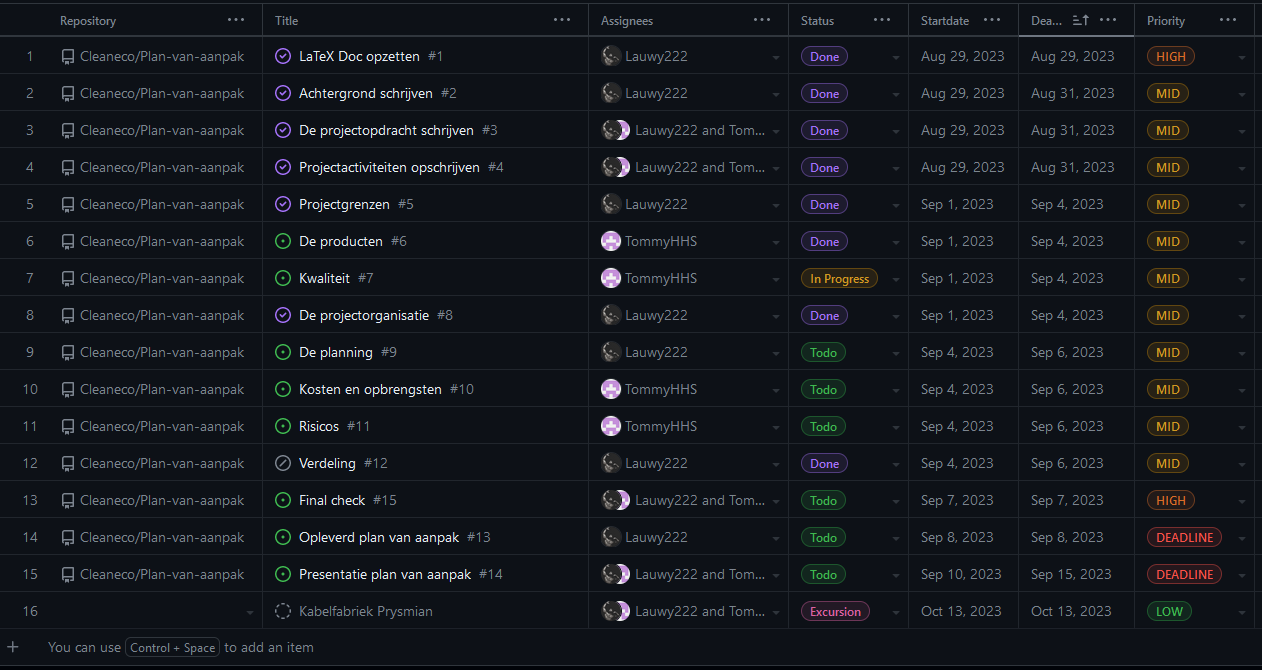
\includegraphics[width=0.9\textwidth]{IMG/overview.PNG}
%     \caption{Overview screenshot vanuit GitHub.}
%     \label{fig:overview}
% \end{figure}

% \newpage
% In de \textbf{ToDoList}\textit{(figuur:\ref{fig:todolist})} worden vier lijsten weergegeven en gecategoriseerd onder vier koppen: Te doen, In uitvoering, Voltooid en Excursie. Hier geven we aan in welke fase van voltooiing elke opdracht zich bevindt, of het nu nog moet worden gedaan, in uitvoering is, is voltooid, of het een excursie betreft die we moeten voorbereiden.

% \begin{figure}[h]
%     \centering
%     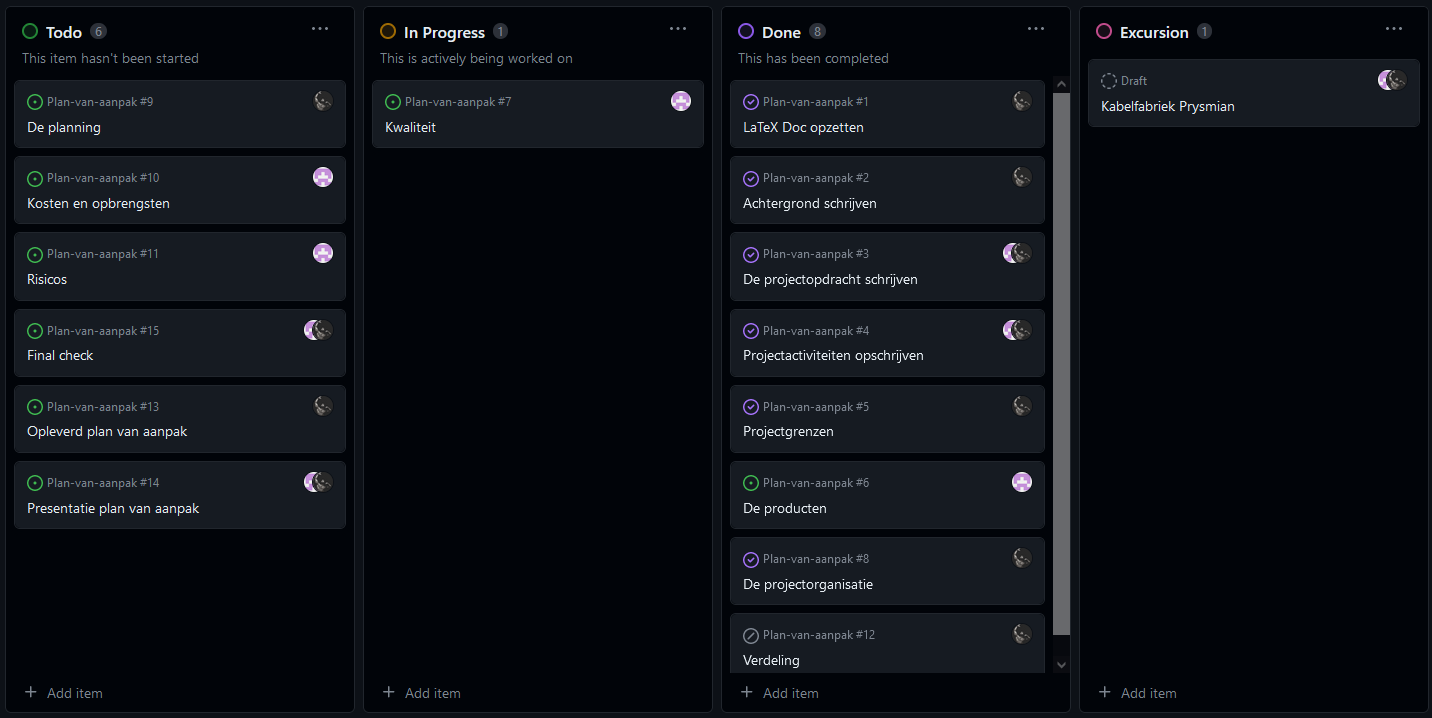
\includegraphics[width=0.9\textwidth]{IMG/todolist.PNG}
%     \caption{ToDoList screenshot vanuit GitHub.}
%     \label{fig:todolist}
% \end{figure}

% De \textbf{Roadmap}\textit{(figuur:\ref{fig:roadmap})} toont visueel wanneer een opdracht had moeten beginnen en wanneer de deadline is.

% \begin{figure}[h]
%     \centering
%     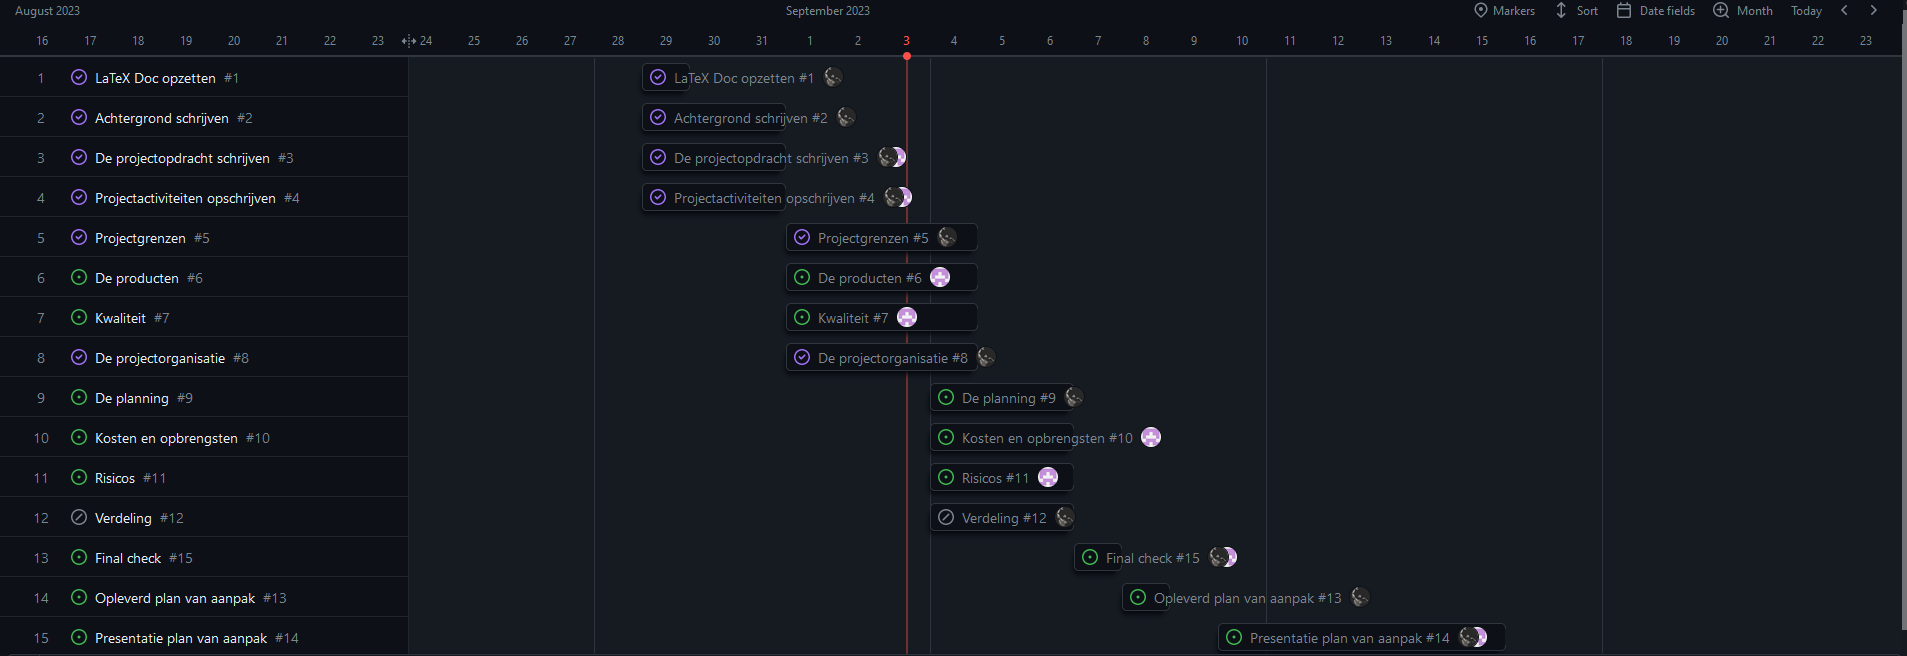
\includegraphics[width=0.9\textwidth]{IMG/roadmap.PNG}
%     \caption{Roadmap screenshot vanuit GitHub.}
%     \label{fig:roadmap}
% \end{figure}
% Als er complicaties optreden tijdens het proces van dit project, kunnen we op tijd een opmerking plaatsen en om hulp vragen. Op deze manier zijn we niet beperkt tot fysieke vergaderingen. We kunnen ook per opdracht aangeven wat niet lukt, waardoor alles nog gestructureerder verloopt.

% OLD

% \section{Planning} \label{planning}
% Wij hebben een planning in Github. Hierin geven wij het volgende aan:

% \textit{- Repository: Aan welk project het onderwerp is gekoppeld}

% \textit{- Title: wat is de titel van de opdracht}

% \textit{- Assignees: wie moet(en) de opdracht maken}

% \textit{- Status: hoe staat het ervoor met de opdracht}

% \textit{- Start-Date en Deadline: wat is de start- en einddatum van de opdracht}

% \textit{- Priority: wat is de urgentie van de opdracht}

% Wij hebben drie verschillende views: Overview, TodoList, Roadmap.

% Bij \textbf{Overview} wordt er een overzicht van alle taken laten zien die al gedaan zijn of nog moeten worden gedaan met extra informatie hierboven genoemd

% Bij \textbf{TodoList} worden er vier lijsten gevisualiseerd geindexeerd door vier kopjes. ToDo, In Progress, Done en Excursion. Hier geven we aan welke opdracht in welke status fase is of dat het een excursie is die wij moeten voorbereiden.

% Bij \textbf{Roadmap} wordt er gevisualiseerd wanneer een opdracht gestart moest zijn en wanneer de deadline is. 


% Mochten er complicaties voorkomen tijdens het process van dit project dan kunnen we optijd een comment plaatsen en vragen om hulp. Zo zijn wij dus niet gelimiteerd aan fysieke meetings. Ook kunnen wij per opdracht aangeven wat er niet lukt en alles dus nog gestructureerder is.


% Elke week worden er opdrachten gemaakt. Bij elke opdracht wordt een begin- en eindtijd gegeven. Het is de bedoeling dat de opdracht binnen deze tijd af is. Zodra dit niet het geval is, zal er eerst in overleg met de groepsleden besproken worden of de eindtijd verschoven mag/kan worden. Als daarentegen de ingeplande tijd voor de betreffende opdracht realistisch was en de opdracht niet af is, zal er in overleg met de opdrachtgever een kort gesprek moeten worden gevoerd om dit in de toekomst te voorkomen. Als er geen verbeteringen te zien zijn in de nabije toekomst, moeten er consequenties worden genomen door de groepsleden en de opdrachtgever.
% Voor de planning wordt Github gebruikt als tool om de opdrachten voor het project duidelijk weer te geven. In figuur 1 is te zien dat één opdracht uit zes kolommen bestaan. Daarin staat de:


% 
\includegraphics[width=6.7in]{IMG/08_planning_01.png} \\
% - Notes: wat moet er worden gedaan om de opdracht te voltooien
% In de opeenvolgende rijen daaronder worden alle opdrachten gemaakt met daarin de bijhorende informatie die in de bovenste kolommen gedefinieerd staan.
% \\\\